\section{Introduction}

Procedural Content Generation (PCG) is a fundamental challenge in computational design, requiring algorithms to produce complex, randomized, yet strictly rule-abiding structures. The Wave Function Collapse (WFC) algorithm, originally introduced by Maxim Gumin in 2016 \cite{gumin2016wave}, elegantly addresses this by framing procedural generation as a formal constraint satisfaction problem. Operating on principles inspired by quantum mechanics, the algorithm initializes a domain where every cell exists in a superposition of all possible states. Through an iterative process of observation and propagation, the algorithm continuously collapses the lowest-entropy cells and strictly enforces adjacency constraints until a globally valid configuration is achieved.

\vspace{1cm}
\begin{figure}[H]
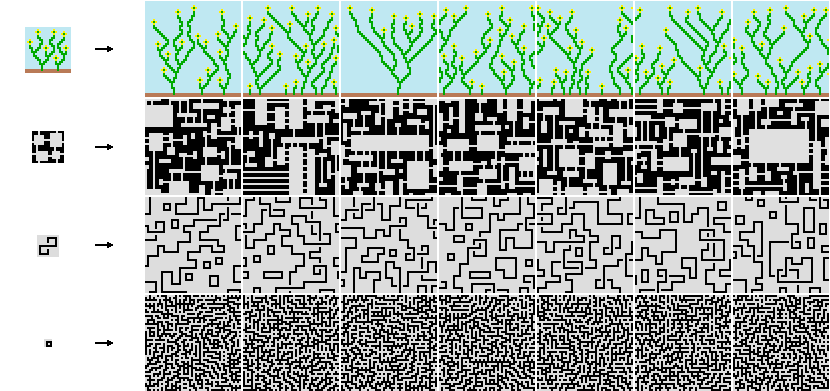
\includegraphics[scale=0.5]{figs/wfc.png}
\caption{Examples from the Maxim Gumin Github repository.}
\end{figure}
\vspace{1cm}

\subsection{Parallel Implementation Challenge}

In recent years, numerous researchers have sought to optimize the computational performance of the WFC algorithm. Notable advancements include the implementation of graph-based data structures to extend WFC beyond rigid spatial grids \cite{kim2019automatic}, as well as the development of hybrid frameworks that combine constraint solving with traditional procedural noise to bypass sequential bottlenecks \cite{buyukcsar2024enhancing}. However, academic literature concerning the direct, distributed parallelization of the core WFC algorithm remains remarkably sparse. This gap is primarily due to the algorithm's inherently non-local constraint propagation: a single cell collapse can trigger a cascading chain reaction of state removals that ripples unpredictably across the entire domain. This creates a highly strict data-dependency structure, where the state of any given cell relies entirely on the successful resolution of constraints originating from distant coordinates. Consequently, true parallel WFC remains a significant and open computational challenge.

To make parallelization feasible, it is strictly necessary to limit the propagation diameter. Once a hard bound on constraint propagation is guaranteed, the computation on a distributed system becomes feasible. In this work, we resolve the sequential bottleneck through a parallel design built upon the Message Passing Interface (MPI). By subdividing the generation domain into nodes and enforcing a policy of exclusive access via mask sliding, we guarantee a conflict-free execution. Crucially, to properly handle the required boundary awareness between adjacent subdomains, our implementation utilizes asynchronous halo-exchange techniques via the MPI interface. This mapping ensures synchronized, overlapping boundary resolution without deadlocks, allowing all nodes to advance in parallel while maintaining the statistical correctness of the final generation.

\subsection{Report Structure}

The remainder of this report is structured as follows. Section 2 details the standard sequential algorithm, establishing the baseline mechanics and strict global data dependencies. Section 3 outlines the parallel design, introducing the conflict-free mask sliding policy. Section 4 presents the topology implementation and the specific tile sets used to limit the propagation bound. Section 5 discusses the technical nuances of the MPI implementation, specifically focusing on domain decomposition, halo exchanges, and centralized data aggregation. Finally, Sections 6, 7, and 8 cover the experimental setup on the CAPRI HPC infrastructure, the execution results, and a critical discussion of the algorithm's scalability limitations and improvements.